\documentclass[hyperref={pdfpagelabels=false}]{beamer}
\usepackage{lmodern}
\usetheme{Frankfurt}
\usepackage{natbib}
\usepackage{apalike}
\usepackage{graphicx}
\usepackage{listings}
\usepackage{caption}
\usepackage{subcaption}
\lstset{basicstyle=\ttfamily, escapeinside={\%*}{*)}}

\title{A Tutorial for \textsc{TIPSI}, and How to Assemble Paths}
\author{Dylan Goldsborough}
\date{8\textsuperscript{th} of July 2016}

\begin{document}
\begin{frame}
\titlepage
\end{frame} 

\begin{frame}
\frametitle{Table of contents}
\tableofcontents
\end{frame} 

%%% Introduction

%% General starting slide
\section{Introduction} 
\setcounter{subsection}{1}
%% Who am I and what did I do?
\begin{frame}
\frametitle{Introduction}
Who am I?
\begin{itemize}
\item Dylan Goldsborough
\item Student at the computational science master
\item Attended the course on biomolecular simulation
\item Enjoyed figuring out \textsc{TIPSI} in class
\item Did a project to write a tutorial that introduces \textsc{TIPSI} over the past months!
\end{itemize}
\end{frame}

%% Structure
\begin{frame}
\frametitle{Outline}
In this presentation I will:
\begin{itemize}
\item Give a brief recap of TPS
\item Outline my contribution
\item Discuss both the examples the tutorial offers
\item Discuss the additional documentation
\end{itemize} 
\end{frame}

\begin{frame}
\frametitle{What is TPS?}
\textbf{Find trajectories of rare transitions}:
\begin{center}
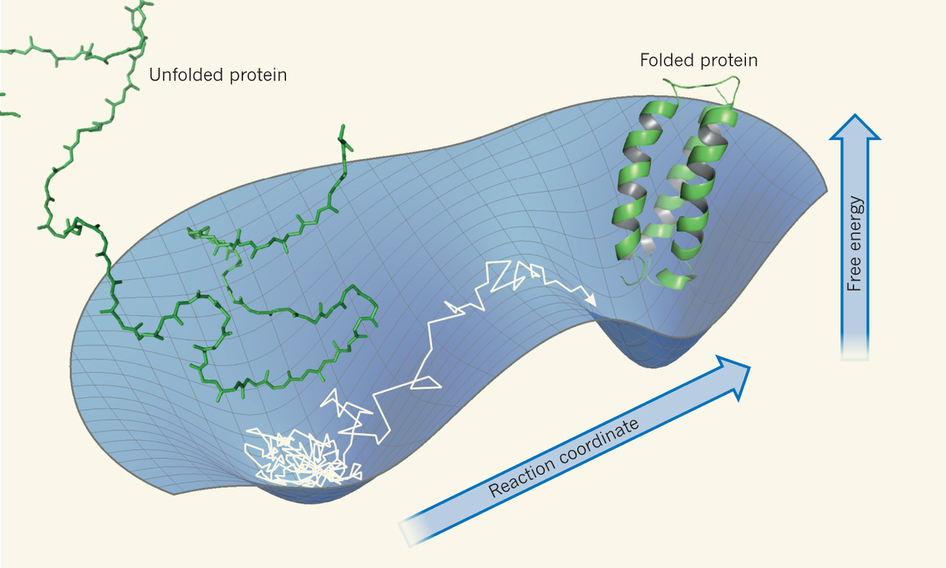
\includegraphics[scale=0.3]{images/fold.png}
\end{center}
(Chung and Eaton, 2013)
\end{frame}

%% What is TPS again?
%% Likely preaching to the coir, so keep it at 5 slides
\begin{frame}
\frametitle{What is TPS?}
Algorithm:
\begin{itemize}
\item Take existing path
\item Choose random time slice \textit{t}
\item Change momenta slightly at \textit{t}
\item Integrate forward or backward in time to create new path
\item Accept if state \textit{A} or \textit{B} is reached, otherwise reject and retain old path
\end{itemize}
\textbf{Important}: we assume that both states are stable, and that we have a transition trajectory ready!
\end{frame}

\begin{frame}
\frametitle{What is TPS?}
\textbf{Committor probability}:
\begin{center}
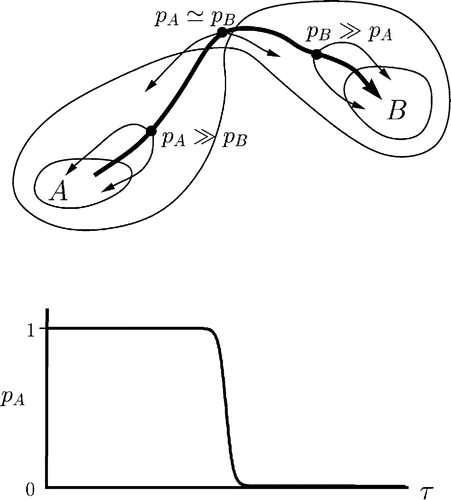
\includegraphics[scale=0.4]{images/bolhuis1.png}
\end{center}
(Bolhuis, 2002)
\end{frame}

\begin{frame}
\frametitle{What is TPS?}
\textbf{Shooting move}:
\begin{center}
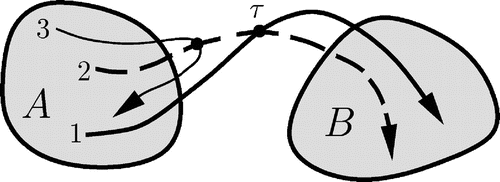
\includegraphics[scale=0.5]{images/bolhuis2.png}
\end{center}
Accepted if state \textit{A} or \textit{B} is reached.\\
(Bolhuis, 2002)
\end{frame}

%% What is TIPSI?
% Redo of a Perl script
% Tsjerk Wassenaar
% Python
% Bit of reverse engineering due to lack of documentation
% Runs GROMACS in reverse time, no reverse velocities, which has pros and cons
\begin{frame}
\frametitle{What is \textsc{TIPSI}?} 
\textsc{TIPSI} is a script by Tsjerk Wassenaar, which:
\begin{itemize}
\item Adaptation of a Perl script by Jarek Juraszek
\item Written in Python
\item It relies on \textsc{GROMACS} version 4.5.4 (a molecular dynamics engine)
\item Does random shooting moves forward and backward
\item Reverses time for backward shooting
\item A "molecular calculator"
\end{itemize}
\end{frame}

%%% What did I write?
\section{Contributions}
\setcounter{subsection}{1}

%% xvg reading and plotting
%% Bash to compile paths, was a bitch
%% Python to analyze metadata
\begin{frame}
\frametitle{Contributions}
I made several minor contributions to this project:
\begin{itemize}
\item Bash implementation to assemble paths
\item Python script to analyze the paths
\item Tutorial with a Python tool
\end{itemize}
Resulted in some surprises that had to be dealt with...
\end{frame}

%% Bash in more detail, how does this work?
\begin{frame}
\frametitle{Assembling paths}
\textsc{Tipsi} only saves the shooting moves to save space, so to view and analyze the transitions we need to assemble them.\\
\textbf{The problem}: 
\begin{itemize}
\item \textsc{TIPSI} outputs shooting moves only
\item Instructions on how the paths are made in \texttt{dat}-files
\item Backward shooting moves are the wrong way around
\item Negative timestamps
\end{itemize}
\textbf{Result}: assembling the paths is a minor nightmare...
\end{frame}

\begin{frame}[fragile]
\frametitle{\textsc{TIPSI} output}
\textbf{Example of \textsc{Tipsi output}}:
\begin{lstlisting}
DIR: tipsi-tutorial/output/jobname/DATA/9/1

9-1-BW.cpt  9-1-BW.out  9-1-BW.xtc  DONE
9-1-BW.dat  9-1-BW.top  9-1.dat     md-prod.mdp
9-1-BW.edr  9-1-BW.tpr  ACCEPTED    PARENT
9-1-BW.err  9-1-BW.trr  CMD         parent.dat
\end{lstlisting}
%\begin{center}
%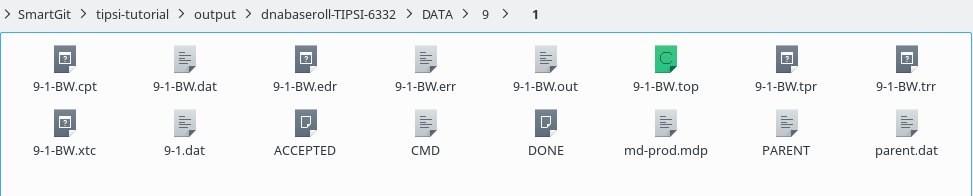
\includegraphics[scale=0.4]{images/outputfiles.png}
%\end{center}
\end{frame}

\begin{frame}[fragile]
\frametitle{\textsc{TIPSI} output}
\begin{lstlisting}
REGEX: '[A-I]\s+(\S+)\s+[F-T][a-z]+\s+(\S+)\s+'

state   time    stop    file
A       -1325.0 True    ../../9/1/9-1-BW.trr
I       -1305.0 False   ../../9/1/9-1-BW.trr
I       -1285.0 False   ../../9/1/9-1-BW.trr
I       -1265.0 False   ../../9/1/9-1-BW.trr
...
I       465.0   False   ../../6/4/6-4-FW.trr
I       485.0   False   ../../6/4/6-4-FW.trr
I       505.0   False   ../../6/4/6-4-FW.trr
B       525.0   True    ../../6/4/6-4-FW.trr
\end{lstlisting}
\end{frame}

%% Mention that GROMACS does not like negative times...
\begin{frame}
\frametitle{Assembling paths}
\textbf{The solution}: 
\begin{itemize}
\item Bashscripts that searches for directories with \texttt{ACCEPTED}-file
\item Scans \texttt{dat}-file using regular expressions
\item Overwrites timestamps
\item Creates each path by dumping and appending single frames
\item Stores some metainformation in a \texttt{csv}-file
\end{itemize}
Takes a while to dump frames for long trajectories...
\end{frame}

%% Python script, what do I plot?
\begin{frame}
\frametitle{Metainformation paths} 
We can do some nice things with the metainformation, I wrote a script that:
\begin{itemize}
\item Finds the average path length
\item Finds the number of decorrelated groups of paths
\item Ratio of FW:BW shooting moves
\item Draws a tree of all shooting moves
\end{itemize}
\end{frame}

%%% Example 1
\section{Example: alanine dipeptide} 
\setcounter{subsection}{1}

%% Introduce the molecules
\begin{frame}
\frametitle{Alanine Dipeptide} 
Our first example is \textbf{alanine dipeptide}:
\begin{itemize}
\item Extremely fast to run
\item Very simple to understand, with simple order parameters (dihedrals)
\item Has a nice transition between two distinct states
\item Common example to use
\end{itemize}
\end{frame}

\begin{frame}
\frametitle{Alanine Dipeptide} 
\begin{center}
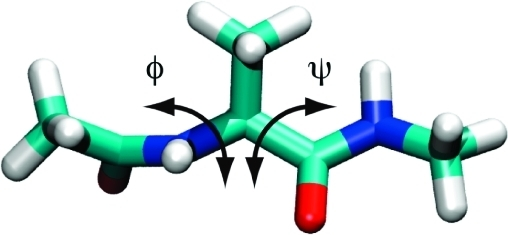
\includegraphics[scale=0.4]{images/alanine.png}
\end{center}
\end{frame}

%% Describe the steps in the tutorial
\begin{frame}
\frametitle{Preparing for \textsc{TIPSI}} 
In this example we do everything from scratch:
\begin{itemize}
\item Start with \texttt{pdb}-file (defines the structure) and MD settings
\item We prepare make a periodic system with a solvent
\item We do energy minimization followed by a constrained MD run
\item We do runs at room temperature and high temperature
\end{itemize}
We look at the order parameters in the run using a Python script and \textsc{Gromacs} commands.
\end{frame}

\begin{frame}
\frametitle{Defining the stable states} 
\begin{figure}[t!]
    \begin{subfigure}[t]{0.5\textwidth}
        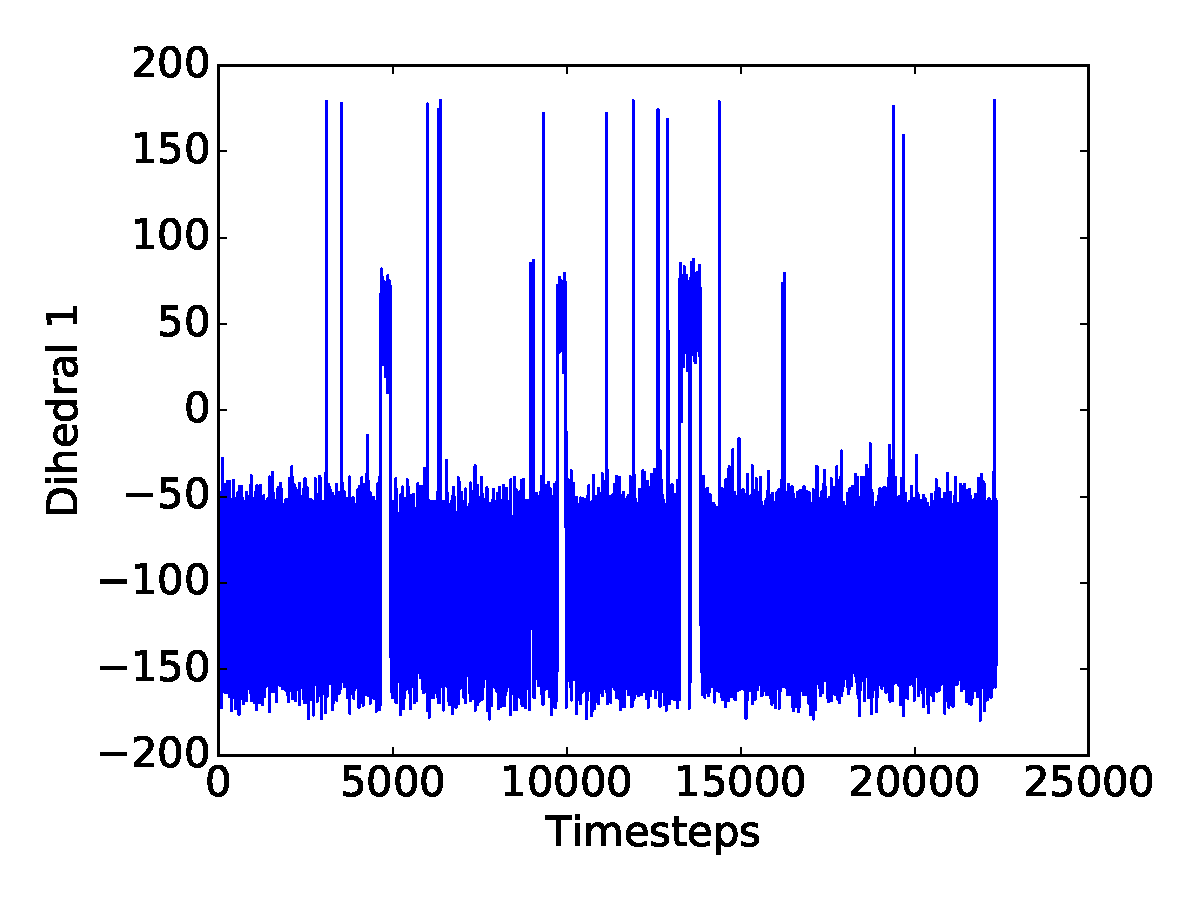
\includegraphics[width=\textwidth]{images/C_Dihedral1.pdf}
    \end{subfigure}%
    \begin{subfigure}[t]{0.5\textwidth}
        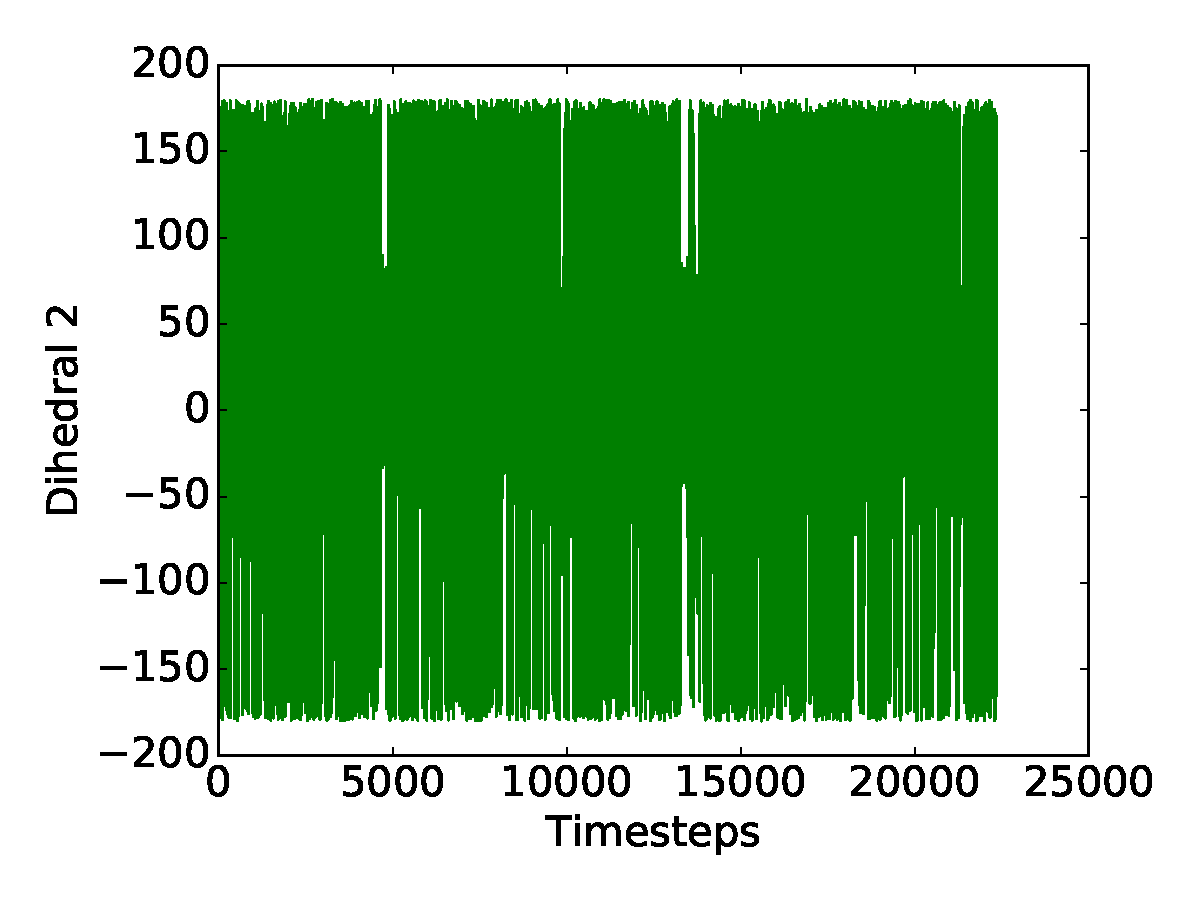
\includegraphics[width=\textwidth]{images/C_Dihedral2.pdf}
    \end{subfigure}
\end{figure}
\end{frame}

\begin{frame}
\frametitle{Defining the stable states} 
\begin{center}
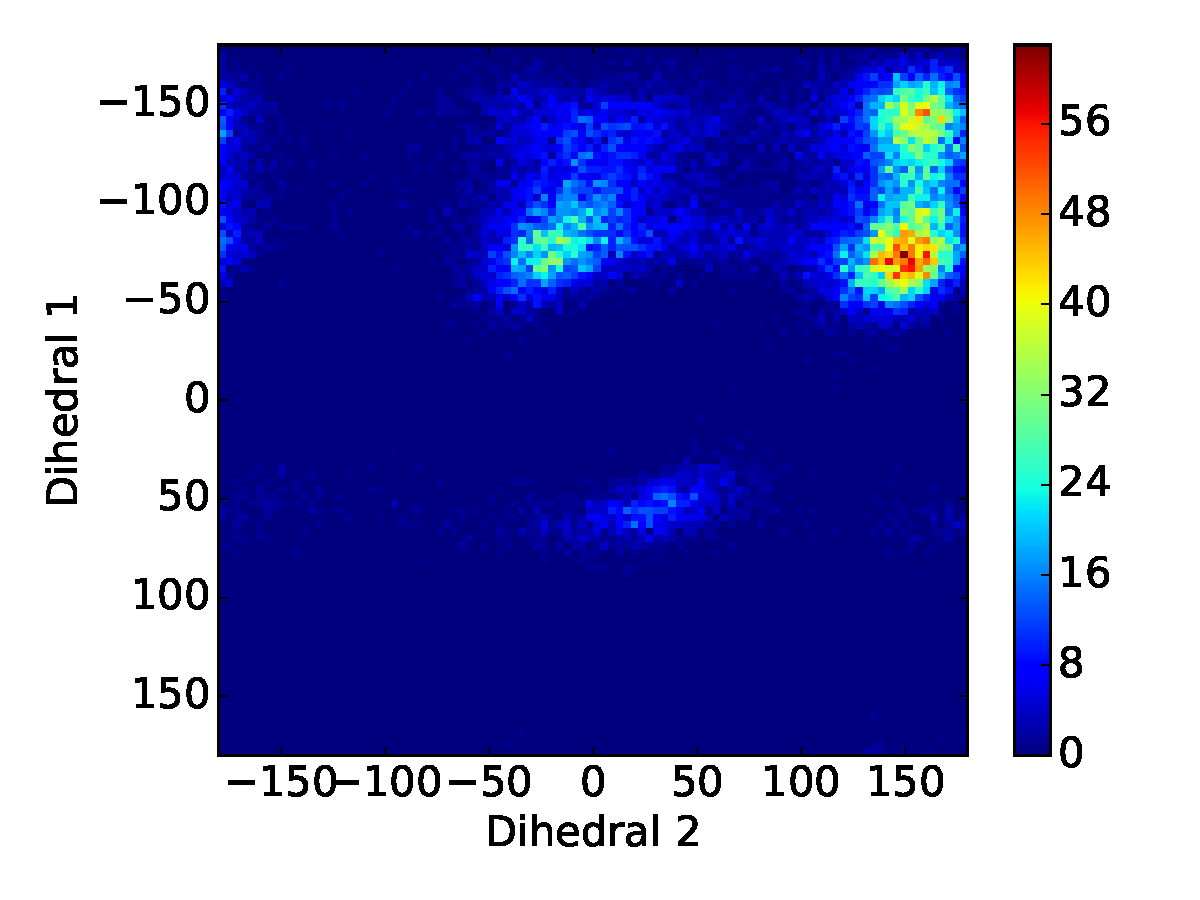
\includegraphics[scale=0.4]{images/C_2D.pdf}
\end{center}
\end{frame}

\begin{frame}[fragile]
\frametitle{Running \textsc{TIPSI}}
\begin{lstlisting}
maxframes  = 2000

par dh1  = dihdeg(frame$Dihedral1)
par dh2  = dihdeg(frame$Dihedral2)

state A = (-150 < dh1 & dh1 < -50 
	& 120 < dh2 & dh2 < 180)
state B = (-100 < dh1 & dh1 < -50 
	& -50 < dh2 & dh2 < 20)

interface I = (!A) & (!B)
\end{lstlisting}
\end{frame}

\begin{frame}
\frametitle{Analyzing \textsc{TIPSI}} 

I appended the bashscript to the end of the job, so that it puts all paths and the metadata in the \texttt{output/DATA} directory, now we can take a look at the trajectory in VMD! 

We find that:

\begin{itemize}
\item Average length is 136.4 frames
\item FW/BW ratio is 0.4
\item Number of decorrelated groups of paths is 2
\end{itemize}

\end{frame}

\begin{frame}
\frametitle{Analyzing \textsc{TIPSI}} 
\begin{center}
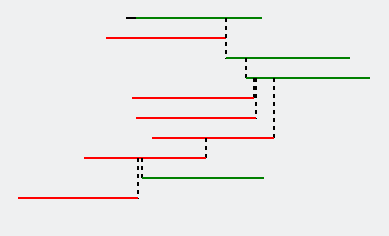
\includegraphics[scale=1]{images/tree.png}
\end{center}
\end{frame}

%%% Example 2
\section{Example: DNA baseroll}
\setcounter{subsection}{1}

%% Introduce what happens 

\begin{frame}
\frametitle{DNA baseroll} 
Second example is the DNA baseroll:
\begin{itemize}
\item Project by Jocelyne Vreede and David Swenson
\item Concerns the transition from the WC- to the HG-pairing
\item An actual rare event (microsecond range), unlike example 1
\end{itemize}
Metadynamics simulation has been done, so there is a trajectory available that contains the transition!
\end{frame}

\begin{frame}
\frametitle{DNA baseroll} 
\begin{center}
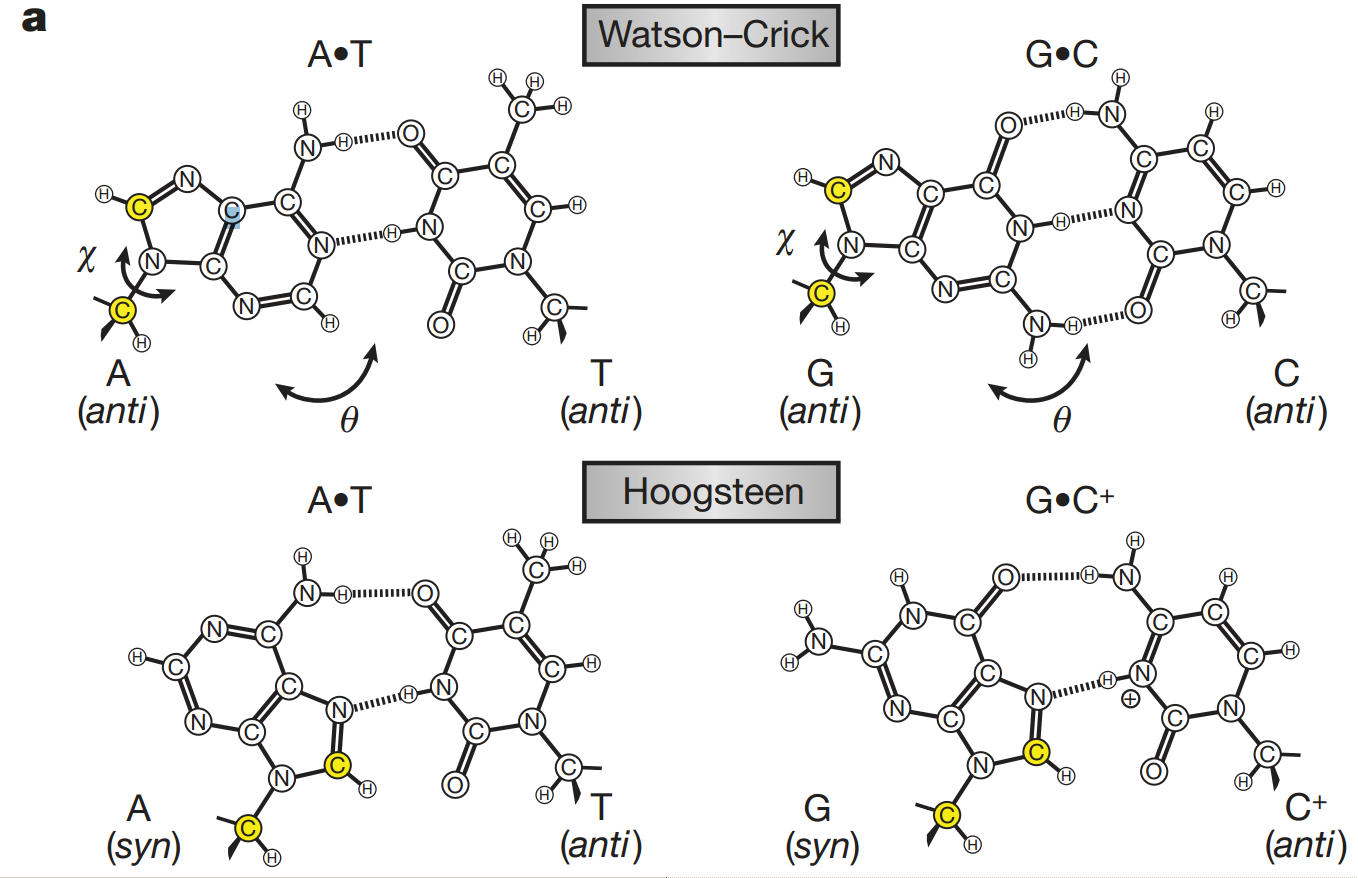
\includegraphics[scale=0.2]{images/pairing.png}
\end{center}
\end{frame}

%% Describe the steps in the tutorial
\begin{frame}
\frametitle{Preparing for \textsc{TIPSI}} 
In this example we start with a trajectory and state definitions:
\begin{itemize}
\item We import the custom topology
\item We create a \texttt{tpr}-file (containing the simulation settings) to suit our MD-needs
\item We set up a parameter file that include the state definitions (H-bonds)
\item We run \textsc{tipsi} with this \texttt{tpr} and the provided trajectory
\end{itemize}
We look at the order parameters in the run using a Python script and \textsc{Gromacs} commands.
\end{frame}

%% Describe the analysis steps
\begin{frame}
\frametitle{Analyzing \textsc{TIPSI}}

(Same slide as with dipeptala, when carbon is up again...)

\end{frame}

%%% Appendices
\section{Appendices}
\setcounter{subsection}{1}

% Linux and GROMACS not very interesting, but included a guide to very basic parameter files
\begin{frame}
\frametitle{Cheatsheets}
As an appendix, I included:
\begin{itemize}
\item A Linux cheatsheet, for students who are unfamiliar
\item A \textsc{gromacs} cheatsheet (which I caught myself use often too)
\item A \textsc{tipsi} cheatsheet
\end{itemize}
The last adresses the documentation problem with \textsc{tipsi}.
\end{frame}

% Problem: non-inclusive of everything, there are probably more options I did not need and had no chance to explore
\begin{frame}
\frametitle{Cheatsheets}
\textsc{tipsi} cheatsheet includes:
\begin{itemize}
\item How to set up a parameter file
\item All calculator options
\item Several ways to define groups of atoms
\begin{itemize}
\item Numpy arrays
\item Groups from \textsc{gromacs} \texttt{ndx}-files (defines groups of atoms by their number)
\end{itemize}
\end{itemize}
There are \textbf{indexing problems}...
\end{frame}

\begin{frame}
\frametitle{Relevant XKCD}
\begin{center}
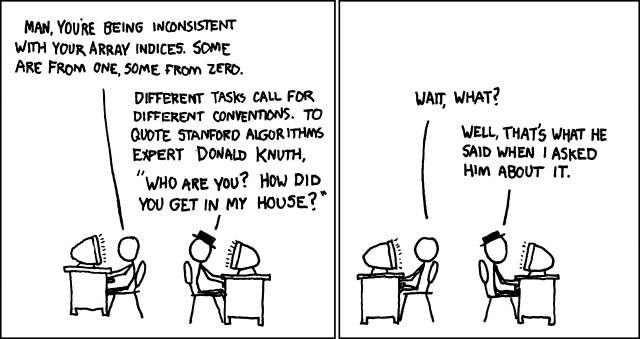
\includegraphics[scale=4]{images/donald_knuth.png}
\end{center}
\end{frame}

\begin{frame}
\frametitle{Running \textsc{TIPSI}} 
Calculator options are:
\begin{itemize}
\item \texttt{com}: center of mass
\item \texttt{dist}: distance (several options)
\item \texttt{angle}: angle of 3 atoms
\item \texttt{dihrad}/\texttt{dihdeg}: dihedral in rads/degrees
\item \texttt{rgyr}: radius of gyration, incompatible with \textsc{gromacs}
\item \texttt{rmsd}: root-mean-square-deviation
\item \texttt{hbonds}: number of hydrogen bonds, specific or non-specific
\end{itemize}
\end{frame}

%%% Summary
\section{Summary}
\setcounter{subsection}{1}

\begin{frame}
\frametitle{Summary} 
\begin{itemize}
\item I wrote a tutorial for students/people interested in \textsc{tipsi} with a fast and uninteresting example, and a more computationally demanding but actually interesting example
\item Added a bash script that finishes the output to make it fit for further analysis
\item Added a basic script that helps understand the shooting moves made
\item Compiled all calculator options, and how to set up a parameter file for \textsc{tipsi}
\end{itemize}
\end{frame}

%% Final slide: I will leave it here, but the project is on GIT and addition can be made
\begin{frame}
\frametitle{Future changes?}
There might be some things to change down the line:
\begin{itemize}
\item Include OPS as an analysis tool (no time now, and still being developed)
\item Append to the possibilities in the parameter file (non-calculator options)
\item Any other changes...
\end{itemize} 
The project is on GIT and should be public: \url{https://github.com/dgoldsb/tipsitutorial.git}
\end{frame}

\end{document}
